%----------------------------------------------------------------------------------------
%	PACKAGES AND OTHER DOCUMENT CONFIGURATIONS
%----------------------------------------------------------------------------------------

\documentclass[12pt]{article} % Default font size is 12pt, it can be changed here

\usepackage{geometry} % Required to change the page size to A4
\geometry{a4paper} % Set the page size to be A4 as opposed to the default US Letter

\usepackage{graphicx} % Required for including pictures

\usepackage{float} % Allows putting an [H] in \begin{figure} to specify the exact location of the figure
\usepackage{wrapfig} % Allows in-line images such as the example fish picture
\usepackage[version=3]{mhchem}
\usepackage{color}

\usepackage{lipsum} % Used for inserting dummy 'Lorem ipsum' text into the template

\linespread{1.2} % Line spacing

%\setlength\parindent{0pt} % Uncomment to remove all indentation from paragraphs

\graphicspath{{pictures/}} % Specifies the directory where pictures are stored

\begin{document}

%----------------------------------------------------------------------------------------
%	TITLE PAGE
%----------------------------------------------------------------------------------------

\begin{titlepage}

\newcommand{\HRule}{\rule{\linewidth}{0.5mm}} % Defines a new command for the horizontal lines, change thickness here

\center % Center everything on the page

\textsc{\LARGE Babraham Institute}\\[1.5cm] % Name of your university/college

\HRule \\[0.4cm]
{ \huge \bfseries PIP3 project}\\[0.4cm] % Title of your document
\HRule \\[1.5cm]

\begin{minipage}{0.4\textwidth}
\begin{flushleft} \large
\emph{Author:}\\
Vladimir \textsc{Kiselev} % Your name
\end{flushleft}
\end{minipage}
~
\begin{minipage}{0.4\textwidth}
\begin{flushright} \large
\emph{Collaborator:} \\
Mounahannad \textsc{Malek} % Supervisor's Name
\end{flushright}
\end{minipage}\\[4cm]

{\large \today}\\[3cm] % Date, change the \today to a set date if you want to be precise

%\includegraphics{Logo}\\[1cm] % Include a department/university logo - this will require the graphicx package

\vfill % Fill the rest of the page with whitespace

\end{titlepage}

%----------------------------------------------------------------------------------------
%	TABLE OF CONTENTS
%----------------------------------------------------------------------------------------

\tableofcontents % Include a table of contents

\newpage % Begins the essay on a new page instead of on the same page as the table of contents 

%----------------------------------------------------------------------------------------
%	Polysome data
%----------------------------------------------------------------------------------------

\section{Role of PTEN/SHIP2 in PI(3,4)P2 metabolism} % Major section

Let us consider a small part of phosphoinositide signaling pathway consisting of PIP3 and PI(3,4)P2 species:

\begin{figure}[H] % Example image
\center{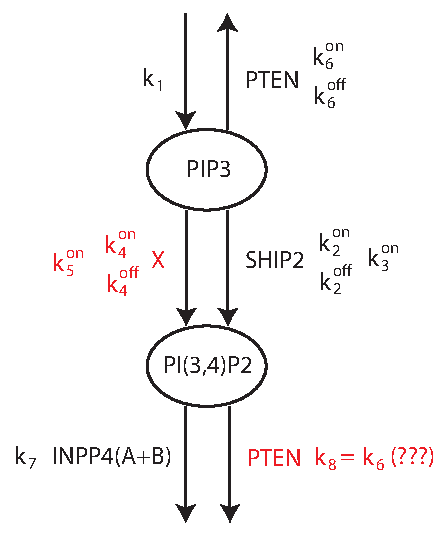
\includegraphics[width=0.5\linewidth]{figures/pip3-pi34p2-diagram.pdf}}
\caption{Diagram of PIP3 and PI(3,4)P2 production and degradation with corresponding reaction constant (see next paragraph). \textcolor{red}{X is an unknown phosphatase that can act together with SHIP2. Role of PTEN in PI(3,4)P2 degradation is validated in the next paragraphs.}}
\label{fig:diagram}
\end{figure}

\subsection{Chemical basis} % Sub-section
Diagram in Fig. \ref{fig:diagram} can be described by the following system of chemical reactions:
\begin{equation}
 \ce{ ->[\ce{k_1}] PIP3}
 \label{eq:pip3_production}
\end{equation}

\begin{equation}
 \ce{PIP3 + SHIP2 <->[\ce{k_2^{on}}][\ce{k_2^{off}}] PIP3\_SHIP2}
 \label{eq:pip3_ship2_binding}
\end{equation}

\begin{equation}
 \ce{PIP3\_SHIP2 ->[\ce{k_3^{on}}] PI_{(3,4)}P2 + SHIP2}
 \label{eq:pi34p2_production_ship2}
\end{equation}

\begin{equation}
 \ce{PIP3 + X <->[\ce{k_4^{on}}][\ce{k_4^{off}}] PIP3\_X}
 \label{eq:pip3_X_binding}
\end{equation}

\begin{equation}
 \ce{PIP3\_X ->[\ce{k_5^{on}}] PI_{(3,4)}P2 + X}
 \label{eq:pi34p2_production_X}
\end{equation}

\begin{equation}
 \ce{PIP3 + PTEN <->[\ce{k_6^{on}}][\ce{k_6^{off}}] PIP3\_PTEN}
\end{equation}

\begin{equation}
 \ce{PI_{(3,4)}P2 + INPP4AB ->[\ce{k_7}] PI_{(3,4)}P2\_INPP4AB}
 \label{eq:pi34p2_degradation_inpp4ab}
\end{equation}

\subsection{PI3K inhibition} % Sub-section

In the presence of 1uMPI-103 PI3K inhibitor \(k_1 = 0\). PIP3 degradation is performed by PTEN, SHIP2 and some other phosphatase X. If additionally assumed that \(k_6^{on}>>k_6^{off}\), \(k_2^{on}>>k_2^{off}\) and \(k_4^{on}>>k_4^{off}\) then changes of PIP3 concentration can be written as:

\[
 \frac{d [PIP3]}{d t} = -[PIP3](k_6^{on}[PTEN] + k_2^{on}[SHIP2] + k_4^{on}[X])
\]

Solution of this equation:

\[
 \frac{d [PIP3]}{[PIP3]} = -dt(k_6^{on}[PTEN] + k_2^{on}[SHIP2] + k_4^{on}[X])
\]

\[
 ln([PIP3]) = -(k_6^{on}[PTEN] + k_2^{on}[SHIP2] + k_4^{on}[X])t + const
\]

\[
 [PIP3] \sim e^{-(k_6^{on}[PTEN] + k_2^{on}[SHIP2] + k_4^{on}[X])t}
\]

Assuming that concentrations of \([PTEN]\), \([SHIP2]\) and \([X]\) are constant:

\begin{equation}
 [PIP3] \sim e^{-(PTEN_{act} + SHIP2_{act} + X_{act})t}
 \label{eq:pip3_theory}
\end{equation}

\subsection{Exponential regression} % Sub-section

\(PTEN_{act}\), \(SHIP2_{act}\) and \(X_{act}\) in equation (\ref{eq:pip3_theory}) can be defined from time courses of PIP3 concentration data (in the presence of 1uMPI-103 PI3K inhibitor). We performed exponential regression of PIP3 data and results are shown in Fig. \ref{fig:regressions}.

\begin{figure}[H] % Example image
\center{\includegraphics[width=0.9\linewidth]{../copasi/inhibitor-regressions.pdf}}
\caption{PIP3 time courses in the presence of 1uMPI-103 PI3K inhibitor. Black lines - regression of the first few time points based on equation (\ref{eq:pip3_theory}).}
\label{fig:regressions}
\end{figure}

Note that time courses of PIP3 concentration have a biphasic behavior and it was not possible to fit all of the data points to a single exponent, thus regression analysis was performed only on a few first time points of the time courses. Regression analysis provides:
\[SHIP2_{act} + X_{act} = 0.0212 [\mu M\cdot s]^{-1}\]
\[PTEN_{act} + X_{act} + \alpha \cdot SHIP2_{act} = 0.0654 [\mu M\cdot s]^{-1}\]
\[X_{act} + \alpha \cdot SHIP2_{act} = 0.0088 [\mu M\cdot s]^{-1}\]

\(\alpha\) is a percentage of active SHIP2 left in the cells after removing it using siRNA (90\% of SHIP2 RNAs are removed). If \(X_{act} = 0\) then \(\alpha \simeq 41.5 \%\). \textcolor{red}{Taking into account that there is a non-linear dependence between active SHIP2 left in the cells and the amount of silenced SHIP2 RNAs (90\%) one could suggest that there is no other phosphatase \(X\) in the pathway and there is still 41.5\% of active SHIP2 left in the cells.}

However, if \(X_{act} \neq 0\) and \(\alpha = 10\%\), then:

\[SHIP2_{act} = 0.0138 [\mu M\cdot s]^{-1}\]
\[X_{act} = 0.0074 [\mu M\cdot s]^{-1}\] 
\[PTEN_{act} = 0.0566 [\mu M\cdot s]^{-1}\]

So that \(X_{act} \simeq 53.6\% SHIP2_{act}\) and \(SHIP2_{act} \simeq 24.4\% PTEN_{act}\)

\subsection{Inconsistency in PTEN KO and SHIP2 silencing} % Sub-section
Experimental data (in the absence of inhibitors) show that removing either PTEN or SHIP2 from the cells increase a peak of PIP3 concentration to \(\sim5 [uM]\). However, in previous section it is shown that activity of PTEN on PIP3 is \(\sim 5\) times higher than that of SIP2 on PIP3. Thus, theoretically it is expected that PTEN will increase the peak of PIP3 to \(\sim1.4-1.5 [uM]\) (checked with COPASI).

\subsection{Is all PI(3,4)P2 produced from PIP3 through SHIP2?} % Sub-section

Let us assume there is no X phosphatase in the pathway in Fig. \ref{fig:diagram}. Then PI(3,4)P2 is produced and degraded as described by equations (\ref{eq:pi34p2_production_ship2}) and (\ref{eq:pi34p2_degradation_inpp4ab}). If INPP4AB is also silenced then PI(3,4)P2 would be only produced as described by equation (\ref{eq:pi34p2_production_ship2}):

\[\ce{PIP3\_SHIP2 ->[\ce{k_3^{on}}] PI_{(3,4)}P2 + SHIP2}\]

where production of PIP3\_SHIP2 complex is described by equation (\ref{eq:pip3_ship2_binding}):

\[\ce{PIP3 + SHIP2 <->[\ce{k_2^{on}}][\ce{k_2^{off}}] PIP3\_SHIP2}\]

In these two reaction there is only information about \(k_2^{on}\) (see chapters above about \(SHIP2_{act}\)). However, one can estimate the maximum production of PI(3,4)P2 by assuming that \(k_3^{on} \gg k_2^{on} \gg k_2^{off}\). In this case two reactions above can be simplified into one:

\begin{equation}
 \ce{PIP3 + SHIP2 ->[\ce{k_2^{on}}] PI_{(3,4)}P2 + SHIP2}
 \label{eq:pi34p2_max_production}
\end{equation}

Note that equation (\ref{eq:pi34p2_max_production}) correspond to the case when the rate of PI(3,4)P2 production is maximal possible. Based on this equation changes of PI(3,4)P2 concentration can be written as:

\[
 \frac{d [PI(3,4)P2]}{d t} = k_2^{on}[SHIP2][PIP3]
\]

Using the definition of \(SHIP2_{act}\) (see equation (\ref{eq:pip3_theory})):

\[
 d [PI(3,4)P2] = SHIP2_{act}[PIP3]d t
\]

And after integration:

\begin{equation}
 [PI(3,4)P2](t) = SHIP2_{act}S_{PIP3}(t) + [PI(3,4)P2](0)
 \label{eq:pi34p2_max_concentration}
\end{equation}

where \(S_{PIP3}(t)\) is the area and the curve of PIP3 time course.

We then calculated the maximum concentration of PI(3,4)P2 produced from PIP3 by SHIP2 using experimental data on PIP3 concentration and equation (\ref{eq:pi34p2_max_concentration}) and compared it with experimental data on PI(3,4)P2 concentration. Results are shown in Fig. \ref{fig:pi34p2_production_no_pten}.

\begin{figure}[H] % Example image
\center{\includegraphics[width=1.0\linewidth]{../copasi/inhibitor-activities-INPP4AB1.pdf}}
\caption{PI(3,4)P2 experimental and theoretical (based on equation (\ref{eq:pi34p2_max_concentration})) time courses.}
\label{fig:pi34p2_production_no_pten}
\end{figure}

It is clear that just SHIP2 is not enough to be able to produce such a high peak of PI(3,4)P2 concentration as shown in Fig. \ref{fig:pi34p2_production_no_pten} (PTEN\(\&\)siINPP4(A+B) condition).

\subsection{Hypothesis: PTEN dephosphorylates PI(3,4)P2 to PI4P} % Sub-section

Transient concentrations of PI(3,4)P2 in PTEN\(\&\)siINPP4(A+B) condition are very large to be controlled by only one phosphotase SHIP2 (see paragraph above). Since in siINPP4(A+B) condition concentration of PI(3,4)P2 does not significantly change, an obvious hypothesis would be that PTEN might be another phosphotase that take a role in dephosphorylation of PI(3,4)P2 to PI4P (see Fig. \ref{fig:diagram}). Thus, when PTEN is knocked out PI(3,4)P2 accumulates faster. However, adding PTEN to PI(3,4)P2 regulation would in theory add an extra outflux (higher than the influx of SHIP2) from PI(3,4)P2 pool. This outflux cannot explain accumulation of PI(3,4)P2 in the absence of PTEN and would completely vanish PI(3,4)P2 in siINPP4(A+B) condition (blue line in Fig. \ref{fig:pi34p2_production_no_pten}). Therefore, there must be another source of PI(3,4)P2 of approximately the same strength as PTEN activity to be able to neutralize PI(3,4)P2 degradation by PTEN in siINPP4(A+B) condition and to accumulate a large amount of it in PTEN\(\&\)siINPP4(A+B) condition (checked with COPASI).

\end{document}

